\usetikzlibrary{calc}
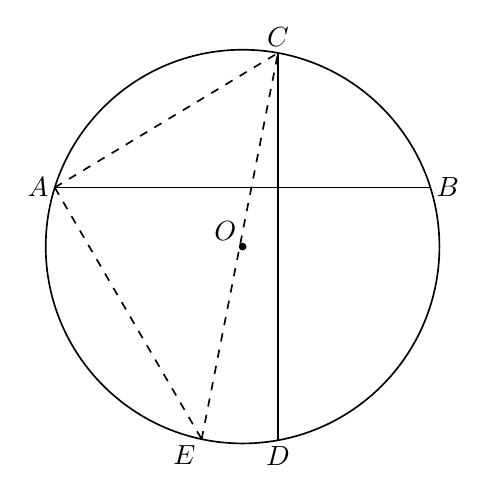
\begin{tikzpicture}[x=1cm,y=1cm,line width=.6pt,font=\normalsize]
\coordinate (O) at (0,0);
\coordinate (A) at (-2.3848,0.75);
\coordinate (B) at (2.3848,0.75);
\coordinate (C) at (0.45,2.4592);
\coordinate (D) at (0.45,-2.4592);
\coordinate (E) at (-0.5198,-2.4454);
\coordinate (P) at (0.45,0.75);
\draw (O) circle[radius=2.5cm];
\draw (A)--(B);
\draw (C)--(D);
\draw[dashed] (A)--(C);
\draw[dashed] (A)--(E);
\draw[dashed] (E)--(C);
\node[left=2pt,inner sep=0pt] at (A) {$A$};
\node[right=2pt,inner sep=0pt] at (B) {$B$};
\node[above=2pt,inner sep=0pt] at (C) {$C$};
\node[below=2pt,inner sep=0pt] at (D) {$D$};
\node[below left=2pt,inner sep=0pt] at (E) {$E$};
\node[above left=2pt,inner sep=0pt] at (O) {$O$};

% Explicit named circle-center points, painted after all region fills.
\fill (O) circle[radius=1.4pt];
\end{tikzpicture}
